% ============================================== %
% PROPOSED METHODS %
% ============================================== %


\subsection{The DiVE-Swap Scheme}
\label{subsec:dive-swap}
The DiVE-Greedy algorithm presented in the previous section is of the constructive type. 
%
That is, it starts with an empty set of views and incrementally constructs it by adding one view at a time. 
%
To the contrary, our DiVE-Swap presented in this section falls under the {\em local search} type of algorithms. 
%
In general, a local search algorithm starts out with a complete initial solution and then attempts to find a better solution in the neighborhood of that initial one. 
%
Like constructive algorithms, local search algorithms are also widely used in solving optimization problems including diversification. 
%
For instance, the Swap local search method has been utilized to maximize diversity \cite{Drosou, Vieira2011, DBLP:conf/sigmod/HussainKS15}, and in this paper, we further expand it to our DiVE schemes. 

The basic idea underlying DiVE-Swap is to start with an initial set $S$ of size $k$ and then iteratively modify the set $S$ in order to improve the value of the objective function $F(S)$. 
%
One of the main design criteria in local search algorithms is the choice of the initial solution. 
%
In DiVE-Swap, we consider two natural variants: 1) {\em DiVE-iSwap}, and 2) {\em DiVE-dSwap}. 
%
In DiVE-iSwap, $S$ is initialized with the $k$ views that maximize importance and can be easily obtained using our baseline Linear-Importance (Sec. ~\ref{subsec:baseline}).
%
Alternatively, in DiVE-dSwap, $S$ is initialized with the $k$ views that maximize diversity using Greedy-Diversity (Sec.~\ref{subsec:baseline}).
%

Apart from the initialization approach, both variants work similarly. 
%
Particularly, in each iteration, each unselected view $X_i \in X$ is interchanged with all views in $S$ (Algorithm \ref{DiVE-Swap} line 9). 
%
\eat{
Particularly, in each iteration, each unselected view $X_i \in X$ is interchanged with all the selected views in $S_j \in S$ (Algorithm \ref{DiVE-Swap} line 9). 
}
%
That is, the overall hybrid objective function is computed as $F(S \backslash S_j \cup X_i)$.  
%
Then the one interchange that leads to the highest new value for $F$ is applied and $S$ is updated accordingly (Algorithm \ref{DiVE-Swap} line 14). 
%
Such iterations are repeated until no more views can be swapped between $X$ and $S$, which is reached when no further improvement is achieved in the value of $F$ (Algorithm \ref{DiVE-Swap} line 17).   


% %explain why initialization by Importance and Initialization by Diversity

In comparison to DiVE-Greedy, DiVE-Swap incurs the same query processing cost $C_Q$. 
%
Furthermore, it incurs even higher $C_D$ cost for computing diversity, which can reach up to $ O\left(kn^2 \right) $. 
%
However, DiVE-Swap offers a valuable opportunity for maximizing the number of pruned views, and in turn reducing the query processing cost $C_Q$, as described in the next section.   

%
%\hak{
%Therefore, it is fair to state that for high dimensional large datasets, the query processing cost for both DiVE-Greedy and DiVE-Swap can easily become a performance bottleneck. To address that challenge, we optimise our proposed DiVE schemes using pruning technique to reduce the number of queries that need to be executed. The details of our pruning scheme are provided in the next section.
%}


\eat{
\mas{\sout{
	Similar to DiVE-Greedy, the cost of DiVE-Swap is dominated by query processing cost $C_Q$ as well.
	%
	However, in the next section, we describes that DiVE-Swap can offers a valuable opportunity for maximizing the number of pruned views, and in turn reducing the query processing cost $C_Q$, which is the dominant factor in determining  efficiency (Sec. ~\ref{subsec:pruning-Greedy-Swap}). 
	}
}  
}










%
%\risch{
%		As mentioned in the previous section, DiVE-Greedy is a constructive algorithm.
%		%
%		In the first iteration, $S$ has a very small number of views (i.e., two most distant views). 
%		%
%		Meanwhile, our context-driven consists of three components (i.e., attribute, measure, and aggregate function) as explained in Sec ~\ref{context-driven-deviation}.
%		%
%		Since the size $S$ is a small and each view consists of three components ($A,M, F$) then many of the remaining unselected views in $X$ are expected to have same score of $ setDist(X_i, S) $.
%		%
%		Hence, this condition can decreases the chance of pruning due to many views are not satisfying the pruning condition (Sec. ~\ref{subsec:pruning-Greedy-Swap}). 
%		%
%		To overcome the limitation of DiVE-Greedy, we propose DiVE-Swap algorithm in this section which falls under the {\em local search} type of algorithms.
%		
%	}
%\eat{
%\hak{As mentioned in the previous section, DiVE-Greedy initializes the set $S$ with two most distant views. Those views are selected soley on the basis of their contextual distance and guide the selection of views in the later iterations. In case the initial two views have low importance score, the value of $F(S)$ is consequently affected adversely. However, as DiVE-Greedy is a constructive algorithm and builds set $S$ iteratively, there is no possibilty of replacing the initially selected views later with high importance views. Hence, to overcome the limitaiton of DiVE-Greedy, we propose DiVE-Swap algorithm in this section which falls under the {\em local search} type of algorithms.} \mas{what does that mean? is that the actual motivation for proposing Swap? So we are proposing Swap to improve effectiveness?!! }
%}
%
%\eat{
% \mas{ \sout{
%%
%As explained in the previous section, DiVE-Greedy starts with small number of views (i.e., two most distant views) in the initialization set $S$ which these views cannnot be replaced. 
%%
%Hence, it may reduce the quality of recommended views due to there is no guarantee that two most distant views in the initialization set $S$ are the most optimal views in terms of $F(S)$.
%%
%Moreover, there is no way to replace these two views. 
%%
%In order to overcome these issues, DiVE-Swap is proposed as well. DiVE-Swap technique has a replacing mechanism that can replace low-utility views in the current set $S$ with the better one.
%}
%}
%%
%\sout{
%	Different from DiVE-Greedy algorithm which is one of the constructive type, our DiVE-Swap presented in this section falls under the {\em local search} type of algorithms. }
%}
%





\eat{
	
	Naturally, our DiVE-Greedy scheme described above will achieve a high pruning power for high values of $\lambda$ (i.e., more emphasis is given to the diversity score $setDist(V_i,S)$).
	%
	However, that pruning power diminishes for low values of $\lambda$ (i.e.,more emphasis is given to importance score $I(V_i)$).
	%
	That discrepancy in performance happens because of two reasons: 
	%
	(1) the constructive and iterative nature of the greedy algorithm, and (2) utilizing the upper bound on importance $I_u$ when computing $maxU(V_i)$. 
	%
	To explain those reasons, recall that the amount of pruning is shaped by the maximum value of $minU(V_i)$.
	%
	Now, consider an extreme case, in which $\lambda = 0.0$. 
	%
	In that case, all values of $minU(V_i)$ will also be equal to zero, and no pruning will take place. 
	%
	Similarly, for low values of $\lambda > 0$, the maximum value of $minU(V_i)$ will still be low, leading to limited pruning. 
	%
	That pruning is further reduced when combined with a high value of $I_u$ as it leads to all views acquiring high $maxU(V_i)$ and cannot be pruned.  
	%
	
	
	In addition, DiVE-Swap has bigger number of views in the initialization set $S$ ($|S|$ = $k$). Meanwhile, higher number of views in the set $S$ can decrease the chance of views in $X$ have same $ setDist $ score.  
	
	To address those limitations, we propose an adaptive scheme for setting $I_u$ in Sec.~\ref{subsec:adaptive-pruning}, and  orthogonally introduce our {\em Swap}-based DiVE scheme next.
}
\eat{
	Since Greedy is constructive type algorithm, it contructs the set S by adding a new candidate view, there is no guarantee that the new view selected in each iteration is the best view for the objective function $F(S)$. It is because the view which has the highest utility score not necessary be the best one that improve the objective function $F(S)$ (e.g: local optimum). To overcome that issue, we proposed other schemes which based on swap technique.
}


\eat{
	Swap is local search type algorithm and it has been known and used to maximize diversity in the literature \cite{Drosou, Vieira2011}. This algorithm starts with a complete initial set $S$, and try to achieve better result by interchanging the remaining views in $X$ to the current set $S$. If a view in $X$ is able to improve objective function value $ F $($ S $), then this view can be joined to the current set and one view in the current set that has the lowest contribution to the $ F $($ S $) will be removed. The details of \textit{DiVE-Swap} algorithm can be seen in Algorithm \ref{DiVE-Swap}.
	
	Due to Swap need a complete initial set, we proposed two types of Swaps which are: 1) \textbf{\textit{DiVE-iSwap} }, the underlying behind this sheme is, it has the initial set from the result of Linear-Importance which is importance score maximized.  2) \textbf{\textit{DiVE-dSwap}} which is quite similar to DiVE-iSwap, however, this scheme is initialized by results of Greedy-Diversity, which is diversity maximized. Those two swaps have different initial set and in each iteration, the candidate view is exchanged from $X$ to the current set $S$ till the $F(S)$ is maximized as given in Eq \ref{objectif_function}. 
}

\eat{
	\textbf{\textit{DiVE-Swap cost}}. The costs of Swap algorithm is also depend on the query execution time $C_Q$ of all possible views and the diversity computation $C_D$. The query cost $C_Q$ is executed only once but the cost is high due to it needs I/O cost. However, the complexity of diversity computation $C_D$ is $ O\left(k^2 \right) $ and the number of distance computation depends on the number of iterations of the swap and the number of views in $X$ which can be seen in Algorithm \ref{DiVE-Swap} line 5. In the worst case, swap algorithm can perform $ O\left(k^n \right) $ iterations. Without any pruning scheme, the cost of \textit{DiVE-iSwap} is same as \textit{ DiVE-dSwap} due to those both schemes are using same technique only different in the initial set. 
}


%
%%% how pruning is done
%
%%% contrast to greedy
%\eat{
%In terms of pruning, two our proposed Swap are quite different. \textit{DiVE-iSwap} utilize the results of Linear-Importance as the initial set. Hence, this algorithm cannot escape from executing all queries due to Linear-Importance needs to execute all possible views to get the results. However, the second proposed swap algorithm, \textit{ DiVE-dSwap} is initialized by the result of Greedy-Diversity. This algorithm does not execute any query to generate the results. Therefore, we can employ pruning technique in \textit{ DiVE-dSwap} by leveraging the properties of importance and diversity.
%
%While in \textit{DiVE-Greedy-Static}, the maximum and minimum bound of importance score are utilized, in this scheme, only maximum bound $I_u$ is used. This \textit{ DiVE-dSwap-Static} also leverage both the importance and diversity score of a candidate view to decide whether a view query should be executed or not. The details \textit{ DiVE-dSwap-Static} technique explained as follows:
%
%\begin{itemize}
%	\item Since the initial set of \textit{ DiVE-dSwap} is the result of Greedy-Diversity, all query views in the initial set need to be executed in order to get the objective function $F(S)$ of the current set $S$. The $F(S)$ of current set will be compared to the new $F(S)$ after exchanging a view as shown in Algorithm \ref{DiVE-Swap} line 9.
%	\item In order to confirm that exchanging process starts from the candidate view that has highest score of diversity, all views in $X$ is sorted based on $ setDist\left(V_i, S\right)  $ before start exchanging view from $ X $ to the current set $S$. This is called as \textit{"top-1"} technique. 
%	\item To start exchanging view, the importance score must be known by executing the query of the candidate view. Instead of executing query view, the maximum bound of importance score is used to compute the utility score of each view as in \textit{DiVE-Greedy-Static} technique. Hence, the result is not the actual utility score but $ maxU' $, which defined as: $ 	maxU'\left(V_i\right)= \left(1-\lambda\right) \times I_u\left(V_i\right) + \lambda \times setDist\left(V_i, S\right) $.
%	\item The exchanging process is started by comparing $F(S)$ of the current set to $F(S)$ of new set as given in Algorithm \ref{DiVE-Swap} lines 9 - 10. The $F(S)$ of new set is computed by Eq \ref{objectif_function} while $ maxU' $ is used as the utility score of candidate view from $ X $.
%	\item If using importance score $I_u$ candidate views in $X$ cannot improve the objective function $F(S)$ to the current set $S$, those views will be pruned. 
%\end{itemize}
%
%This technique is valid due to if the maximum score of importance $I_u$ is used and that view cannot improve $F(S)$ of the current set, then there is no reason to execute the view query to get the importance score $I$ ($I \leq I_u$) . 
%
%%This pruning scheme is called \textbf{\textit{DiVE-dSwap-Static}}.
%
%All proposed pruning techniques including \textit{DiVE-Greedy-Static} and \textit{DiVE-dSwap-Static} are using static value $I_u$ as the bound. However, the pruning performance cannot be optimal while the value of $I_u$ is far away from the actual maximum of importance score in database. To overcome this issue, we proposed adaptive pruning scheme as described in the next section. 
%}
%










% Compare with Greedy in terms of pruning performance%

%\subsection{Adaptive Pruning Scheme}
%%Premble
%
%Two pruning techniques \textit{DiVE-Greedy-Static} and \textit{DiVE-dSwap-Static} have been presented. Those two static pruning techniques utilized maximum bound $I_u$ to determine whether the query view need to be executed or not. Only view that can improve the $F(S)$ of the current set while using $I_u$ will be executed otherwise those are pruned. However, one drawback using static bound $I_u$ in pruning technique is that if the bound is far away from the maximum score of importance score in the dataset, the pruning cannot work optimal. To overcome this issue, instead of using static bound $I_u$, we proposed adaptive pruning scheme that automatically adapts the bound to the real maximum importance score in the dataset. 
%
%The adaptive pruning technique is utilizing the maximum bound $I_u$ as in static pruning as a first initial bound, however, this bound is changed to the real value of maximum importance score after some query views are executed. The problem occurs when the executed views have a small importance score and it is far below from the most views in the dataset. Thus, it brings the pruning out of control because while the bound is very low and there are many views in dataset have higher importance score compared to the bound, it may result wrong prune. Hence, DiVE needs the strategy to ensure that the bound score is close as possible to the maximum importance score in the dataset while it is changed. One of the approach that can be used is by selecting sample views to be executed then get the maximum importance score of the view from those sample. This brings us to the question of how many samples are needed in order to hit a view that has a maximum score from the dataset.
%
%There are several literatures have been mentioned related to the confidence interval and the number of samples in the normal distribution [cite]. However, the importance score of candidate views in $X$ is not in normal distribution. The highest importance score is the upper bound of maximum importance $I_u$ whereas the lowest is 0, and it is long tail distribution. Hence, we adopt the sampling method from this [cite] as our data is not in normal distribution, it is called as prediction interval ($ PI $) which is similar to a confidence interval in normal distribution. The relation between $ PI $ and the number of samples defined as in equation \ref{prediction-interval}.
%
%\begin{equation}
%	PI= \dfrac{\left(N-1\right) }{\left(N + 1\right)}, where\, N = Number\, of\, samples
%	\label{prediction-interval}
%\end{equation}
%
%In general, analyst may use $ PI $ start from 80 to 99. While $ PI $ = 80\% states that there are 9 sample views need to be executed, 85 \%, 90\%, 95\%, 97\%, and 99\% means 12, 20, 40, 60, and 200 samples need to be executed respectively. 
%
%\textit{Adaptive pruning flows}. We employ adaptive pruning technique to both schemes, \textit{DiVE-Greedy} and \textit{DiVE-dSwap}. In case of Greedy technique, the upper bound $I_u$ is used at the first time, thus the value $I_u$ is changed to maximum importance score from the samples of views which are executed. In order to change the bound value, the number of samples that need to be executed depends on the $ PI $ value which defined by the analyst. Futhermore, the bound is changed while in the next view execution that there is a view which has importance score higher than the used current bound.
%
%For adaptive pruning technique in \textit{DiVE-dSwap}, the details is described as follows:
%
%\begin{itemize}
%	\item Firstly, as in \textit{ DiVE-dSwap-Static} that all query view in the initial set are executed in order to get the objective function $F(S)$ of the current set $S$ and all candidate views in $X$ is sorted based on $ setDist\left(V_i, S\right)  $.
%	\item $ maxU' $ of each view is computed by utilizing the maximum bound of importance score $I_u$, where $ maxU'\left(V_i\right)= \left(1-\lambda\right) \times I_u\left(V_i\right) + \lambda \times setDist\left(V_i, S\right) $. 
%	\item All views in $X$ is exchanged to the current set one by one and a view that can improve $F(S)$ will be executed in order to get the actual value of importance. 
%	\item The bound is changed while the number of views which are executed reaches the number of sample based on the PI which determined by analyst. For instance, analyst may use PI = 97\%, hence, bound is changed while the sum of number of candidate views and th number of views in the initial set equal to 60 views. While it reaches to 60 views, the bound is replaced by the maximum importance score of executed views.  
%	\item If in the next query view execution, there is a view which has higher importance score than the bound. Thus, the bound is changed to that score. 
%\end{itemize}
%
%%To check the performance of our proposed pruning techniques
%
%In this work, adaptive pruning in Greedy is called \textit{DiVE-Greedy-Adaptive} wheras in Swap is called \textit{DiVE-dSwap-Adaptive}.

%
%
%$maxU'$ of each candidate view is computed first using $current bound$ before executing the query, view which cannot make an improvement to the S while using $current bound$ will never be executed and it will be pruned
%  
%In order to get better performance of pruning scheme, instead of using static $max_I = \sqrt{2} $, we proposed Adaptive Pruning scheme, that can adapt the value of $max_I$ to the real values in the dataset. In order to estimate the $max_I$ which can close to the real value in the dataset, we use sampling method. 


%For instance, in the \textit{DiVE-dSwap-Adaptive-Pruning}, $max_I$ is initialized by $ \sqrt{2} $. If the view by using $max_I$ can improve the objective function value in the current set $S$, the real Importance score of this view will be computed which is by executing the query of its view. For instance, after executing its query, the real Importance value is 0.25, by using $ \alpha= 0.8 $, the $ EWMA_t  $ will be $ (0.8 *0.25) + ((1- 0.4)*\sqrt{2}) = 0.48 $, and the current $max_I$ will be set to 0.48, and it will be updated continuously. This EWMA method able to set the value of $max_I$ as close as the real values in the dataset, it should make pruning scheme works better. 

% % Pruning Pseudocode

%\begin{algorithm}
%	%	\SetAlgoLined
%	%	\KwIn{Set of views V and result set $S$ize k }
%	%	\KwOut{Result set $ S \geq V $, |S| = k}  
%	%	$S \leftarrow $ Result set of only importance or only diversity\;
%	%	$X \leftarrow  \left[V \backslash S\right]$\;
%	%	$F_{current} \leftarrow 0 $\;
%	%	$  improve \leftarrow  True $\;
%	$ max_b  \leftarrow\sqrt{2} $\;
%	%$ X' \leftarrow [] $\;
%	\For{$i$ in set $X$}{
%		\For{$j$ in set $S$}{
%			$ d  \leftarrow setDist\left(X[i],S \backslash S[j]\right) $\;
%			$ 	newX \leftarrow [S[j], X[i], d]$\;
%			$ 	X'.append(newX)$\;
%		}
%	}
%	$ 	X' \leftarrow sorted\_by\_d(X') $\;
%	$ S' \leftarrow S $\;
%	\eIf{ $ max_b == \sqrt{2} $}{
%		\For{$i$ in set $X'$}{
%			
%			\If{ $ F\left(S'\right) < F\left(S \backslash X'[i][0] \cup X'[i][1], max_b\right) $}{
%				$ 	X''.append(X'[i][1])$\;
%			}
%		}
%		
%		$n \leftarrow pi - len(S)$\;
%		$samples \leftarrow X''[0\colon n]$\;
%		$maxI\_S \leftarrow get\_maxI(S)$\;
%		$maxI\_samples \leftarrow get\_maxI(samples)$\;
%		
%		\If{ $ maxI\_S > maxI $}{
%			$ maxI \leftarrow maxI\_S$
%		}
%		\If{ $ maxI\_samples> maxI $}{
%			$ maxI \leftarrow maxI\_samples$
%		}
%		$max\_b \leftarrow maxI$	
%		
%		\For{$i$ in set $X''$}{
%			\For{$j$ in set $S$}{
%				\If{ $ F\left(S'\right) < F\left(S \backslash S[j] \cup X''[i], max_b\right)  $}{
%					$ 	X'''.append(X''[i])$\;
%					$ I \leftarrow get\_I\_score(X''[i]) $\;
%					\If{ $ F\left(S'\right) < F\left(S \backslash S[j] \cup X''[i], I\right) $}{
%						$ S'  \leftarrow S \backslash j \cup X''[i] $  \;
%					}
%					\If{ $ I > max_b $}{
%						$ max_b \leftarrow I $
%					}
%				}
%			}
%		}
%		
%	}{ 
%	\For{$i$ in set $X'$}{$ .... $
%		%			\If{ $ F\left(S'\right) < F\left(S \backslash X'[i][0] \cup X'[i][1]\right) $}{
%		%				$ 	X''.append(X'[i][1])$\;
%		%			}
%		%			$ I \leftarrow get\_I\_(X''[i]) $\;
%		%			\If{ $ F\left(S'\right) < F\left(S \backslash S[j] \cup X''[i], max\_bound\right) $}{
%		%				$ S'  \leftarrow S \backslash j \cup X''[i] $  \;
%		%			}
%		%			\If{ $ I > max\_bound $}{
%		%				$ max\_bound \leftarrow I $
%		%			}
%		
%	}
%	
%}
%
%\If{ $ F\left(S'\right) > F\left(S\right) $}{
%	$ S  \leftarrow S'$
%}
%return S
%\caption{\textit{DiVE} SwapD Pruning}\label{DiVE-dSwap-Pruning}
%\end{algorithm}

%In order to apply pruning in \textit{DiVE-dSwap}, as in the Greedy technique, we utilize the maximum bound of importance score $I_u$ to compute $ maxU' $ of each candidate views in $X$ which defined as:
%In each iteration, instead of computing a complete utility score for each view, only partial utility score is computed, as in equation \ref{partial_utility}. The partial utility score using actual value of diversity score and estimated value of importance score $max_I$ which is equal to $\sqrt{2}$.

%\begin{figure}
%	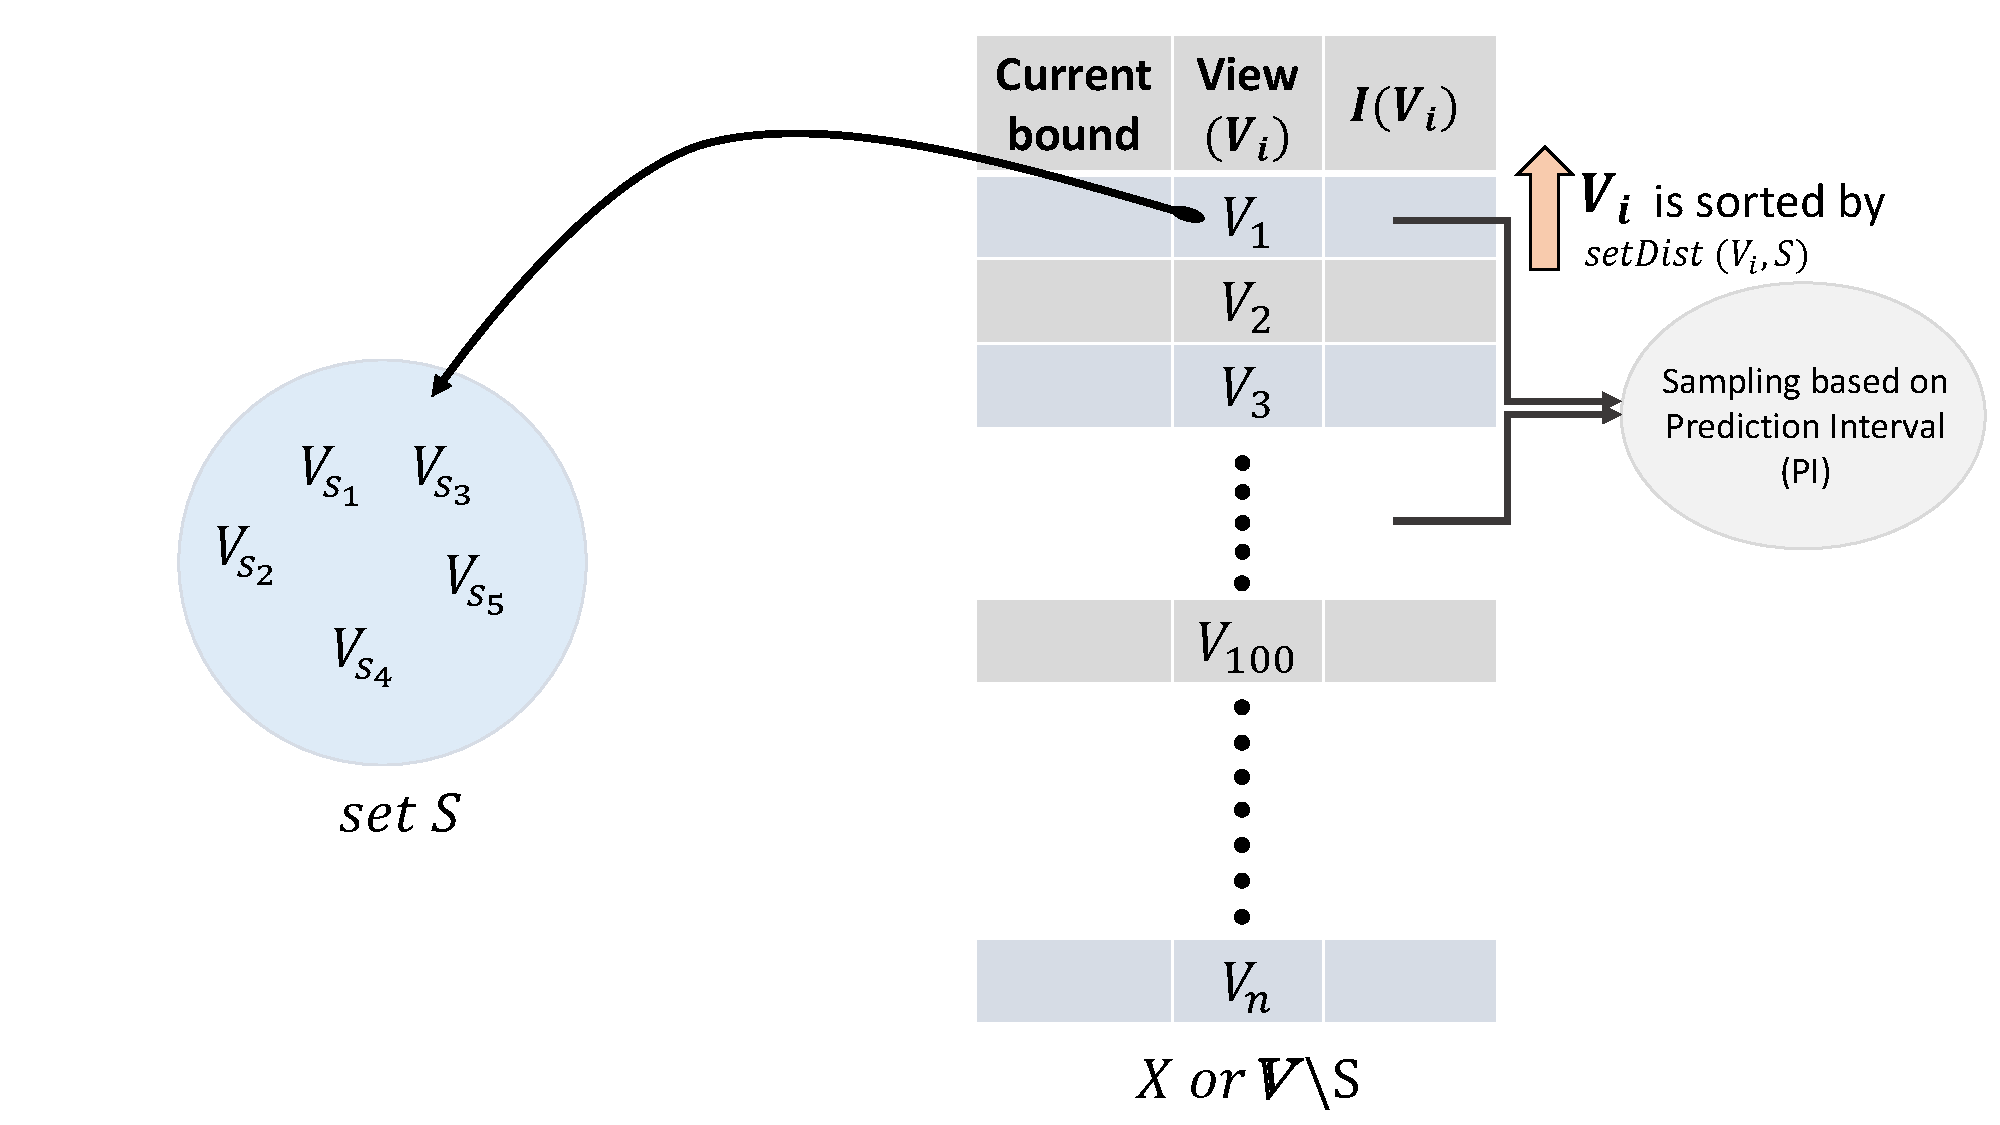
\includegraphics[width=3in]{figures/results/dSwap-Pruning}
%	\caption{dSwap-Pruning: Each candidate view has importance score and $ current bound $. The importance score of view will be generated only for view which its utility score is able to improve set $S$ while using $currentbound$ }
%	\label{fig:dSwap-Pruning}
%\end{figure}

%The idea behind pruning scheme is to minimize the query execution, which is by early prune low quality views. There are two main parameters in pruning scheme: 1) weight of $\lambda$ and 2) the max bound value $I_u$. 

%The weight of $\lambda$ is important due to it determines the contribution of importance score and diversity score. For instance, assume that an analyst wants to get set of views from view recommendation and she uses $\lambda$ = 0.7. The $\lambda$ value equal to 0.7 means that the diversity contribution to the utility score is 70\% and the contribution of importance score will be 30 \%, as it can be seen in equation \ref{objectif_function}. Thus, by setting the $\lambda$ to higher value, the contribution of importance score will be lower and more queries are pruned. This $\lambda$ value is determined by analyst, however, in this experiement 0.5 is used as the default. 